% mainfile: Refinement.tex
%%% =============================================== Preamble BEGINN =====================================================================
%% Lade:
% Dokumentenklasse
\documentclass[
	draft,	% Zeigt nur Rahmen f"ur Bilder an
	english,%german,
	12pt,		% Schriftgr"o"se 11 Arial oder 12 Times New Roman
	%fleqn,	% fleqn für Matheumgebungen linksb"undig
		% Layout:
	open=right,    % vor dem chapter eine leere linke Seite
	twoside,	% zweiseitiges
	a4paper,	% Papierformat
	%normalheadings,
	%DIV=calc, % berechnet mit \typearea[current]{calc} den richtigen Seitendivisor für die Rasterung der Satzspiegels
	%DIV11,
	%BCOR5mm % Bindekorrektur, was weiß bleibt beim druck und nicht für die Berechnung des Satzspiegels benützt wird
	%left=3cm, % max 4
	%right=3cm, % max 4
	%top=2cm, % max 3
	%bottom=2cm % max 3,
	enabledeprecatedfontcommands
] {scrreprt}		% Art des Dokumentes

% Pakete
% for better fitting on a4 paper
%\usepackage{a4} % kein guter Stil
% Umlaute erm"oglichen
\usepackage[utf8]{inputenc}
% Erm"oglicht beim markieren/kopieren des Textes auch die Umlaute
% au"serdem funktioniert damit auch das Trennen von W"ortern mit Umlauten
% Dadurch aber sehr h"assliche Schrift und Schriftbild, aber mit \usepackage{lmodern}
% l"asst es sich wieder heile machen
\usepackage[T1]{fontenc}
% bindet neue Schriften ein und l"asst das Dokument wieder vom Schriftbild normal aussehen
% was durch \usepackage[T1]{fontenc} zerst"ort wurde
\usepackage{lmodern}
% Neue Rechtschreibung %english f"ur Bibliographie

% Index
\usepackage{index}
% Berechnungen mit Befehlen
%\usepackage{calc}
% deutsches Literaturverzeichnis
%\usepackage{babelbib}
% sprachabh"angiges Datum
\usepackage[english,ngerman]{isodate}
% Einzelne Seiten landscape anzeigen
%\usepackage{lscape}
% Tabellen rotieren k"onnen
%\usepackage{rotating}
% F"ur etwas besser einstellbare Listen
%\usepackage{enumerate} kann weniger als enumitem
%\usepackage{enumitem}

% letztes Argument legt die Sprache des Dokuments fest
%\usepackage[english,ngerman]{babel}
\usepackage[english]{babel}
% Eigentlich veraltet, aber babel kann anscheinend keine richtige Silbentrennung
\usepackage{ngerman}
% F"ur Seitenlayout und Darstellung (vorallem eigener Seitenstil) und header und footer
\usepackage[automark,headsepline]{scrpage2}

% f"ur den Zeilenabstand
\usepackage{setspace}
% f"ur farbigen Text
\usepackage{color}
\usepackage{xcolor}
% Times Roman (Microsoft's Times New Roman)
%\usepackage{txfonts}
% Helvetica (Microsoft's Arial)
%\usepackage{helvet}
% Matheumgebungen
%\usepackage{amsmath}
\usepackage{amssymb}
%\usepackage{amsfonts}
%\usepackage[mathcal]{euscript}
%\usepackage{mathrsfs}
%\usepackage{MnSymbol} % attention overwrites many math symbols for example the frown is very short an object with ^ appear very low.
%% for xLeftarrow and so on and mathclap for spaces
\usepackage{mathtools}
% for a fat ;
\usepackage{stmaryrd}
% f"ur nicefrac
\usepackage{units}
% der Shuffle Operator
\usepackage{shuffle}
%\usepackage{amsthm}
% f"ur die theoreme
\usepackage[amsmath,amsthm,thmmarks]{ntheorem}

% Bilder
%% zwei Bilder in einer Umgebung
%\usepackage{subfig} putt
%\usepackage{subfigure} putt
%\usepackage{subcaption}
% Graphiken einbinden
%\usepackage{graphicx}

% Tabellen
% Um zeilenweise Tabellen zu formatieren
%\usepackage{hhline}
% Tabellen mit einstellbarer Breite
%\usepackage{tabularx}
% Tabellen "uber mehrere Seiten
%\usepackage{longtable}
% passt longtable so an, dass auch die Eigenschaften von tabularx verwandt werden k"onnen
%\usepackage{ltxtable}
% Entzerrt Tabellenzeilen
%\usepackage{booktabs}
% Tabellen farblich markieren
%\usepackage{colortbl}
% Figuren und tables mit "H" exakt an einen Platz binden
\usepackage{float}


% Glossar
%\usepackage[ngerman]{translator}
\usepackage[english]{translator}
\usepackage[
	nowarn,       %stop glossar warninings
	nonumberlist, %keine Seitenzahlen anzeigen
	acronym,      %ein Abkürzungsverzeichnis erstellen
	toc]          %Einträge im Inhaltsverzeichnis
{glossaries}

%Umgebung für Code-Fragmente
\usepackage{listings} \lstset{	
	morecomment=[s][\color{darkred}]{"}{"},
	escapeinside={\%*}{*)},
	commentstyle=\color{cdc_Green},
	keywordstyle=\color{blue},
	frame=single,
	backgroundcolor=\color{lstColor},
	breaklines=true,
	tabsize=4
}


% f"ur Hyperlinks
\usepackage[
	plainpages=false,
	pdfpagelabels,
	breaklinks=true,
	a4paper,
	bookmarks,
	bookmarksopen=true,
	bookmarksnumbered=true,
	pdfauthor={Muhammad Ekbal Ahmad},
	pdftitle={Transformational semantics of the combination pi-OZ for mobile processes with data},
]{hyperref}

% f"ur for-Schleifen
%\usepackage{forloop}
% f"ur if-then-else
\usepackage{ifthen}
% for margins foot header titlepage
\usepackage[a4paper]{geometry}

% TODO notes
%\usepackage[disable]{todonotes} % notes not showed
\usepackage[draft]{todonotes}   % notes showed

% Lorem ipsum blindtext \lipsum or lipsum[n]
\usepackage{lipsum}

% Block comments
%\usepackage{comment}
\usepackage{verbatim}

% Seitenlinien
%\usepackage{framed}
%\usepackage{mdframed}

%% Tikz
\usepackage{pgf}
\usepackage{tikz}

% Neue Befehle
% fix \bf issue
\DeclareOldFontCommand{\bf}{\normalfont\bfseries}{\mathbf}
\DeclareOldFontCommand{\sf}{\normalfont\bfseries}{\mathbf}

% Punkte auch bei section
%\renewcommand\l@section{\@dottedtocline{1}{1.5em}{2.3em}}

% buffer commands
%\newcommand\todo[1]{{\marginpar{\color{red}TODO: #1}}}
%\newcommand\todoI[1]{{\color{red}TODO: #1}}
\newcommand\bla{\todo[inline]{Erkl"arung/Beschreibung/F"ulltext}}
%\newcommand\lorem{Lorem ipsum dolor sit amet, consetetur sadipscing elitr, sed diam nonumy eirmod tempor invidunt ut labore et dolore magna aliquyam erat, sed diam voluptua. At vero eos et accusam et justo duo dolores et ea rebum. Stet clita kasd gubergren, no sea takimata sanctus est Lorem ipsum dolor sit amet.}

% partition commands
\newcommand{\newpart}[1]{{\color{darkred}\noindent\rule{0.5\textwidth-1cm}{1pt} #1 new \rule{0.5\textwidth-1cm}{1pt}}\newline}
\newenvironment{old}[1]
{
	\ifthenelse{\boolean{show_all}}{
		\begin{color}{darkgreen}
		\par\noindent\rule{\textwidth}{1pt}
		\begin{center}\underline{#1}\end{center}
	}{\comment{}}
}
{
	\ifthenelse{\boolean{show_all}}{
		\par\noindent\rule{\textwidth}{1pt}\newline
		\end{color}
	}{\endcomment{}}
}
\newenvironment{new}{
%   \begin{mdframed}[outerlinewidth=2,leftmargin=10,%
%     rightmargin=-10pt,backgroundcolor=white,hidealllines=true,leftline=true,%
%     innertopmargin=0pt,splittopskip=\topskip,skipbelow=\baselineskip,innerbottommargin=0pt%
%     skipabove=\baselineskip]%
	%\begin{leftbar}
%\def\FrameCommand{\vrule width 1pt \hspace{1cm}}%
%\MakeFramed {\advance\hsize\width \FrameRestore}
	\marginpar{\color{darkred}\rule{0.5cm}{1pt} $\downarrow$new \rule{0.5cm}{1pt}}
} {
	\marginpar{\color{darkred}\rule{0.5cm}{1pt} $\uparrow$new \rule{0.5cm}{1pt}}
%\endMakeFramed
	%\end{leftbar}
	%\end{mdframed}
}
% Notizen die bei druckversion nicht angezeigt werden
\newcommand\note[1]{\ifthenelse{\boolean{print_media}}{}{{\color{darkgreen}<Note: #1>}}}

% Referenzieren
\newcommand{\refDef}[1]{Definition~\ref{#1}}
\newcommand{\refFig}[1]{Figure~\ref{#1}}
\newcommand{\refSec}[1]{Section~\ref{#1}}
\newcommand{\refChap}[1]{Chapter~\ref{#1}}
\newcommand{\refLem}[1]{Lemma~\ref{#1}}
\newcommand{\refTheo}[1]{Theorem~\ref{#1}}
\newcommand{\refConv}[1]{Convention~\ref{#1}}
\newcommand{\refConj}[1]{Conjecture~\ref{#1}}
\newcommand{\refEq}[1]{Equation~\ref{#1}}
\newcommand{\refEx}[1]{Example~\ref{#1}}
\newcommand{\refCor}[1]{Corollary~\ref{#1}}
% Referenzieren auf Textstelle
%\newcommand\fullRef[1]{Abschnitt \ref{#1} \glqq\nameref{#1}\grqq{} auf Seite~\pageref{#1}}
%% Referenz auf Bild
%\newcommand\imgRef[1]{Abbildung \ref{#1} auf Seite~\pageref{#1}}
%% Referenz auf Tabelle
%\newcommand\tabRef[1]{Tabelle \ref{#1} auf Seite~\pageref{#1}}
%% Referenz auf Definition
%\newcommand\defRef[1]{Definition \ref{#1} auf Seite~\pageref{#1}}

%Funktionale Anforderungen
%\newcounter{functCounter}
%\newcounter{subFunctCounter}[functCounter]
%\renewcommand\thesubFunctCounter{\Alph{functCounter}\arabic{subFunctCounter}}

%\newcommand\functRequirementPackage{
%\refstepcounter{functCounter}
%\setcounter{subFunctCounter}{0}
%}
%\newcommand\functRequirement[4][\empty]{%%% \empty: Standardwert des optionalen Parameters
%\refstepcounter{subFunctCounter}
%\begin{description}
%\itemsep-0.7cm
%\item[\thesubFunctCounter:] #2 \label{fa_\thesubFunctCounter}
%\item[Eingabe:] #3
%\item[Ausgabe:] #4
%\ifthenelse{\NOT\equal{#1}{\empty}}%%
%		{\item[Optional:] #1}%%
%{}
%\end{description}
%}

% Absatz
%\newcommand\abs{\par\medskip}

% Fetter Index
\newcommand{\findex}[2][\empty]{%%% \empty: Standardwert des optionalen Parameters
	\ifthenelse{\equal{#1}{\empty}}%%
		{\index{#2}\emph{#2}}%%
		{\index{#1}\emph{#2}}%%
	}

% In enumerate-Umgebung (a) solche item
\newcommand{\alphaEnums}{\renewcommand{\labelenumi}{(\alph{enumi})}}

%% Mathematik
\newcommand{\nin}{\not\in}
% Elementzeichen mit anschlie"sendem Mengenzeichen
\newcommand\isin{\in \mathbb}
% Potenzmenge
\newcommand{\pom}[1]{\mathbb P\left(#1\right)}
% Komplexe Zahlen
\newcommand\K{\mathbb C}
% Reelle Zahlen
\newcommand\R{\mathbb R}
% Rationale Zahlen
\newcommand\Q{\mathbb Q}
% Ganze Zahlen
\newcommand\Z{\mathbb Z}
% Nat"urliche Zahlen
\newcommand\N{\mathbb N}
% Kaligraphische Zeichen
\newcommand\calN{\mathcal N}
\newcommand\calL{\mathcal L}
%% backard-Matrix
%\newcommand\B{\mathbb B}
%% forward-Matrix
%\newcommand\F{\mathbb F}
% Menge
\newcommand{\set}[2][\empty]{%%% \empty: Standardwert des optionalen Parameters
	\ifthenelse{\equal{#1}{\empty}}
		{\left\{#2\right\}}
		{\left\{#2\; \mid \; #1 \right\}}
}
\newcommand{\pair}[2]{(#1,#2)}
  
\newcommand{\setmulti}[2][\empty]{%%% \empty: Standardwert des optionalen Parameters
	\ifthenelse{\equal{#1}{\empty}}
		{\bigl\{#2\bigr\}}
		{\bigl\{#2\; \mid \; #1 \bigr\}}
}
\newcommand{\card}[1]{\left|#1\right|}
% Betrag
%\newcommand{\betrag}[1]{\left\lvert #1 \right\rvert}
% Das zu zeigen - Zeichen ZZ
%\newcommand{\zz}{Z\kern-.3em\raise-0.5ex\hbox{Z}:}
% Kongruenz
%\newcommand{\kong}[3]{#1\equiv#2\; mod \;#3}
%\newcommand{\inkong}[3]{#1\nequiv#2\; mod \;#3}
% Vektoren
%\newcommand{\vect}[1]{
%	\left(\begin{array}{c}
%			#1
%		\end{array}
%	\right)
%}
% Matritzen
%\newcommand{\mat}[2]{
%	\left(\begin{array}{#1}
%			#2
%		\end{array}
%	\right)
%}

%% Petri-Netz
% Pre-/Postset
\newcommand{\preset}[1]{{^\bullet{}#1}}
\newcommand{\postset}[1]{{#1^\bullet{}}}

% scalable arrows
\makeatletter
\def\slashedarrowfill@#1#2#3#4#5{%
  $\m@th\thickmuskip0mu\medmuskip\thickmuskip\thinmuskip\thickmuskip
   \relax#5#1\mkern-7mu%
   \cleaders\hbox{$#5\mkern-2mu#2\mkern-2mu$}\hfill
   \mathclap{#3}\mathclap{#2}%
   \cleaders\hbox{$#5\mkern-2mu#2\mkern-2mu$}\hfill
   \mkern-7mu#4$%
}
% already defined in mathtools
%\makeatother
%\makeatletter
%\renewcommand{\xLeftrightarrow}[2][]{\ext@arrow 0359\Leftrightarrowfill@{#1}{#2}}
%\makeatother
%\makeatletter
%\renewcommand{\xleftrightarrow}[2][]{\ext@arrow 0359\leftrightarrowfill@{#1}{#2}}
%\makeatother
%\makeatletter
%\renewcommand{\xLeftarrow}[2][]{\ext@arrow 0359\Leftarrowfill@{#1}{#2}}
%\makeatother
%\makeatletter
%\renewcommand{\xRightarrow}[2][]{\ext@arrow 0359\Rightarrowfill@{#1}{#2}}
%\makeatother
%\makeatletter
\newcommand*{\simfill@}{\arrowfill@\cdot\sim\succ}
\newcommand{\xsimrightarrow}[2][]{\ext@arrow 0359\simfill@{#1}{#2}}
\makeatother
%% negations
\makeatletter
\newcommand*{\nrightarrowfill@}{\slashedarrowfill@\relbar\relbar{\raisebox{.12em}{\tiny/}}\rightarrow}
\newcommand{\nxrightarrow}[2][]{\ext@arrow 0359\nrightarrowfill@{#1}{#2}}
\makeatother

\newcommand{\functText}[1]{\mathtt{#1}}

\newcommand{\ebnf}{\;\bigm|\;}
\newcommand{\gdw}{\mathrm{iff}}
\newcommand{\falls}{\mathrm{if}}
\newcommand{\eq}[1]{\stackrel{#1}{=}}
\newcommand{\pref}[1]{\functText{pref}(#1)}
\newcommand{\conj}[1]{\overline{#1}}
%\newcommand{\true}{\functText{true}}
%\newcommand{\false}{\functText{false}}

%% pi-calculus
\newcommand{\names}{\calN}
\newcommand{\relNames}{\mathfrak{N}}
\newcommand{\conames}{\overline{\calN}}
\newcommand{\labels}{\calL}
\newcommand{\actions}{\functText{Act}}
\newcommand{\outA}{\functText{Out}}
\newcommand{\inA}{\functText{In}}
\newcommand{\boutA}{\functText{Bout}}
\newcommand{\picalc}{$\pi$-calculus}
\newcommand{\syntdef}{::=}
\newcommand{\define}{=_{\mathrm{def}}}
\newcommand{\fnF}{\functText{fn}}
\newcommand{\bnF}{\functText{bn}}
\newcommand{\fn}[1]{\functText{fn}(#1)}
\newcommand{\bn}[1]{\functText{bn}(#1)}
\newcommand{\nF}{\functText{n}}
\newcommand{\n}[1]{\functText{n}(#1)}
\newcommand{\subF}{\functText{sub}}
\newcommand{\objF}{\functText{obj}}
\newcommand{\bindF}{\functText{bind}}
\newcommand{\sub}[1]{\functText{sub}(#1)}
\newcommand{\obj}[1]{\functText{obj}(#1)}
%\newcommand{\objbn}[1]{\functText{obj}_\functText{bn}(#1)}
\newcommand{\bind}[2]{\functText{bind}(#1,#2)}
\newcommand{\bnsubstF}{\functText{bn}_{\functText{subst}}}
\newcommand{\bnsubst}[3]{\functText{bn}_{\functText{subst}}(\subs{#1}{#2},#3)}
\newcommand{\struc}{\equiv{}}
\newcommand{\struct}[2]{#1\struc{}#2}
% sequences
\newcommand{\seqset}[1]{\functText{seq}(#1)}
\newcommand{\eseq}{\langle\rangle}
%\newcommand{\seq}[1]{\langle#1\rangle}
\newcommand{\seqconc}[2]{{#1}^{\,\frown{}\,}{#2}}
\newcommand{\seqcom}[2]{#1\leftrightharpoons{}#2}
\newcommand{\subsetsim}{\mathrel{\substack{\textstyle\subset\\[-0.5ex]\textstyle\sim}}}
\newcommand{\simcirc}{\mathrel{\substack{\textstyle\sim\\[-0.4ex]\textstyle\circ}}}
\newcommand{\ec}[1]{\left[#1\right]}%_{\alpha}}
\newcommand{\bigstep}[1]{\xRightarrow{#1}}
\newcommand{\len}[1]{\#(#1)}
%\newcommand{\parl}[1]{\overrightarrow{#1}}
\newcommand{\parl}[1]{\vec{#1}}
\newcommand{\substF}{\sigma}
\newcommand{\subst}[1]{\left(#1\right)\sigma}
%\newcommand{\subs}[2]{\left\{\nicefrac{#1}{#2}\right\}}
\newcommand{\substitue}[2]{\left\{\nicefrac{#1}{#2}\right\}}

% prefix
\newcommand{\singleout}[1]{\bar{#1}}
\newcommand{\out}[2]{\overline{#1}\langle#2\rangle}
\newcommand{\outa}[2]{\overline{#1}\langle#2\rangle}
\newcommand{\bout}[2]{\overline{#1}(#2)}
\newcommand{\bouta}[2]{\overline{#1}(#2)}
\newcommand{\inp}[2]{#1(#2)}
\newcommand{\inpa}[2]{#1\,#2}
% processes
\newcommand{\procs}{\mathcal P^{\pi}}
\newcommand{\sums}{\procs_{M}}
\newcommand{\procsesf}{\procs_{\functText{esf}}}
\newcommand{\procsresf}{\procs_{\functText{resf}}}
\newcommand{\procsrecf}{\procs_{\functText{recf}}}
\newcommand{\procchoice}[2]{#1 + #2}
\newcommand{\procsum}{\sum_{i\in I}{\pi_i.P_i}}
\newcommand{\procpar}[2]{#1 \mid #2}
%\newcommand{\procres}[3][\empty]{%%% \empty: Standardwert des optionalen Parameters
%	\ifthenelse{\equal{#1}{\empty}}{
%		\ifthenelse{\equal{#2}{\empty}}{
%			\textnormal{\underline{\texttt{new}}}
%		}{
%			\textnormal{\underline{\texttt{new}}}\,#2\;#3
%		}
%	}{
%		\textnormal{\underline{\texttt{new}}}\,#2\left(#3\right)
%	}
%}
\newcommand{\procres}[3][\empty]{%%% \empty: Standardwert des optionalen Parameters
	\ifthenelse{\equal{#1}{\empty}}{
		\ifthenelse{\equal{#2}{\empty}}{
			\underline{\functText{new}}
		}{
			\underline{\functText{new}}\,#2\;#3
		}
	}{
		\underline{\functText{new}}\,#2\left(#3\right)
	}
}
\newcommand{\proccall}[2]{#1\langle#2\rangle}
\newcommand{\procdef}[2]{#1(#2)}
\newcommand{\proczero}{\mathbf{0}}
% substitution
\newcommand{\transp}[2]{\left\{#1\leftrightarrow{}#2\right\}}% substitution
\newcommand{\transpT}[2]{\theta_{#1}(#2)}
\newcommand{\supp}[1]{\functText{supp}(#1)}
\newcommand{\cosupp}[1]{\functText{cosupp}(#1)}
% alpha conversion
\newcommand{\alphaeq}{=_\alpha}
% transitions
%% sangiorgi
\newcommand{\transs}[1]{\xrightarrow{#1}}
\newcommand{\intrans}[2]{\transs{\inpa{#1}{#2}}}
\newcommand{\outtrans}[2]{\transs{\out{#1}{#2}}}
\newcommand{\bouttrans}[2]{\transs{\bout{#1}{#2}}}
\newcommand{\tautrans}{\transs{\tau}}
%% mine
\newcommand{\trans}[1]{\xsimrightarrow{#1}}
%\newcommand{\trans}[1]{\rightsquigarrow}
\newcommand{\transin}[2]{\trans{\inp{#1}{#2}}}
\newcommand{\transout}[2]{\trans{\out{#1}{#2}}}
\newcommand{\transbout}[2]{\trans{\bout{#1}{#2}}}
\newcommand{\transtau}{\trans{\tau}}
% rules name, pr"amisse1, pr"amisse2, konklusion, optional Anwendungsbedingung
\newcommand{\kalRule}[5][\empty]{%%% \empty: Standardwert des optionalen Parameters
	\underline{\scriptstyle#2}:\;
	\ifthenelse{\equal{#3}{\empty}}{
		\ifthenelse{\equal{#4}{\empty}}{
			\dfrac{}{#5}
		}{
			\dfrac{#4}{#5}
		}
	}{
		\dfrac{#3 \quad #4}{#5}
	}
	\ifthenelse{\NOT\equal{#1}{\empty}}{\;\;#1}{}
}
% names of rules
\newcommand{\rulename}[1]{$#1$}
\newcommand{\etau}{\rulename{E-TAU}}
\newcommand{\ecall}{\rulename{E-CALL}}
\newcommand{\eout}{\rulename{E-OUT}}
\newcommand{\ein}{\rulename{E-IN}}
\newcommand{\esuml}{\rulename{E-SUM_L}}
\newcommand{\esumr}{\rulename{E-SUM_R}}
\newcommand{\eres}{\rulename{E-RES}}
\newcommand{\eparl}{\rulename{E-PAR_L}}
\newcommand{\eparr}{\rulename{E-PAR_R}}
\newcommand{\eopen}{\rulename{E-OPEN}}
\newcommand{\ecoml}{\rulename{E-COM_L}}
\newcommand{\ecomr}{\rulename{E-COM_R}}
\newcommand{\eclosel}{\rulename{E-CLOSE_L}}
\newcommand{\ecloser}{\rulename{E-CLOSE_R}}
% strong / weak Bisimulation
\newcommand{\sbisim}{\sim}
\newcommand{\wbisim}{\approx}
\newcommand{\simu}{\mathcal{S}}
\newcommand{\weaksimuset}[2]{\simu^{#1,#2}}
\newcommand{\simuset}{\weaksimuset{P}{Q}}
% denotational semantics
\newcommand{\tr}{\functText{Traces}}
\newcommand{\trI}[1]{\mathcal{T_I}(\ec{#1})}
\newcommand{\tracesI}[3]{\mathcal T_{#1}(\ec{\procpar{#2}{#3}})}
\newcommand{\traces}[1][\empty]{
		\ifthenelse{\equal{#1}{\empty}}
		{\mathcal T}
		{\mathcal T(\ec{#1})}
}

\newcommand{\tracesR}[1]{\mathcal{T}_\relNames(\ec{#1})}

\newcommand{\res}[3]{\functText{res}(#1,#2,\traces[#3])}
\newcommand{\failures}[1][\empty]{
		\ifthenelse{\equal{#1}{\empty}}
		{\mathcal F}
		{\mathcal F(#1)}
}
\newcommand{\fd}[1][\empty]{
		\ifthenelse{\equal{#1}{\empty}}
		{\mathcal{FD}}
		{\mathcal{FD}(#1)}
}
% refinement
\newcommand{\refi}[1][\empty]{
		\ifthenelse{\equal{#1}{\empty}}
		{\,\sqsubseteq_{\mathcal T}\,}
		{\,\sqsubseteq_{\mathcal{#1}}\,}
}
\newcommand{\rrefi}[1][\empty]{
		\ifthenelse{\equal{#1}{\empty}}
		{\,\sqsupseteq_{\mathcal T}\,}
		{\,\sqsupseteq_{\mathcal{#1}}\,}
}

% Header/Footer
% style
%\pagestyle{scrheadings}
\pagestyle{empty} % first empty, then until introduction scrheadings
% Konfiguration der Kopf- und Fu"szeilen: siehe scrguide.pdf Kapitel 5 (ab Seite 214)
% pagenumber first roman until introduction arabic
\pagenumbering{Roman} 

% Settings
% Variable je nach dem wie sie gesetzt ist, wird die Druckversion beziehungsweise die digitale Version erstellt
% Bedeutet Links farbig oder schwarz
\newboolean{print_media}
\setboolean{print_media}{false}

% Ob alle Teile angezeigt werden sollen
\newboolean{show_all}
\setboolean{show_all}{false}
%\includecomment{myComment}

%\KOMAoption{BCOR}{7mm}
%\KOMAoption{parskip}{yes}
\KOMAoption{toc}{bib,index,listof}

% Abstand itemize "andern
%\setitemize{itemsep=-0.5cm}

% Seitenränder
\geometry{
	includehead,
	includefoot,
	inner=3cm, % min 3 max 4
	outer=3cm, % min 3 max 4
	top=2cm, % min 2 max 3
	bottom=2cm % min 2 max 3
}
%\geometry{showframe}

% Farben
\definecolor{gruen}{rgb}{.10, .4, .50}
\definecolor{blau}{rgb}{.2, .2, 0.6}
\definecolor{grau}{gray}{.75}
%\definecolor{white}{gray}{.75}
\definecolor{lstColor}{rgb}{0.901,0.901,0.901} %% Back (Almost White)
\definecolor{darkred}{rgb}{0.601,0.001,0.001} %% dunkles Rot
\definecolor{darkgreen}{rgb}{.10, .4, .20}% dunkelgruen
\definecolor{cdc_Blue}{rgb}{0.0,0.355,0.652} %% Heading Blue (Oldenburg CD Ultramarine)
\definecolor{cdc_BlueM}{rgb}{0.25,0.473,0.722} %% Heading Blue Medium (Oldenburg CD Ultramarine 60%)
\definecolor{cdc_BlueL}{rgb}{0.5,0.589,0.793} %% Heading Blue Light (Oldenburg CD Ultramarine 20%)
\definecolor{cdc_Green}{rgb}{0.390,0.695,0.285} %% Heading Green (Oldenburg CD Chartreuse)
\definecolor{cdc_GreenM}{rgb}{0.559,0.758,0.438} %% Heading Green Medium (Oldenburg CD Chartreuse 60%)
\definecolor{cdc_GreenL}{rgb}{0.688,0.828,0.605} %% Heading Green Light (Oldenburg CD Chartreuse 20%)
\definecolor{color_back}{rgb}{0.941,0.941,0.941} %% Back (Almost White)

% Zeilenabstand
\onehalfspacing
% Index
%\newindex{default}{idx}{ind}{Index}
%\newindex{name}{adx}{and}{Namensverzeichnis}
%\newindex{defi}{ddx}{dnd}{Definitionsverzeichnis}
%\newindex{satz}{sdx}{snd}{Satzverzeichnis}
%\newindex{lem}{ldx}{lnd}{Lemmataverzeichnis}
%\newindex{kor}{kdx}{knd}{Korollarverzeichnis}
%\newindex{bemerkung}{bdx}{bnd}{Bemerkungsverzeichnis}
%\newindex{beispiel}{bsdx}{bsnd}{Beispielverzeichnis}

%Einstellungen Code-Fragmente
%\lstset{
%  xleftmargin=13pt,
%  xrightmargin = 5pt,
%  basicstyle=\small\ttfamily,
%  columns=fullflexible,
%  showstringspaces=false,
%  commentstyle=\color{gray}\upshape,
%  literate={"a}{\"a}1 {"o}{\"o}1 {"u}{\"u}1 {"s}{\ss}1
%  {"A}{\"A}1 {"O}{\"O}1 {"U}{\"U}1
%}

%\lstloadlanguages{Java }

%% Listingstyles
\lstdefinelanguage{pseudocode}
{
	alsolanguage=Java,
	morekeywords=[1]{INPUT, OUTPUT, then, od, in, fi, foreach, begin, end, endfor, endforeach, endwhile},
	morecomment=[s][\color{darkred}]{"}{"},
	escapeinside={\%*}{*)},
	commentstyle=\color{cdc_Green},
	keywordstyle=\color{blue},
	frame=single,
	backgroundcolor=\color{white},
	xleftmargin=5pt,
	xrightmargin = 5pt,
	breaklines=true,
}
%\lstdefinelanguage{apt}
%{
%	alsolanguage=Java,
%	morekeywords=[2]{Place, Transition, Arc, Flow, PetriNet, TransitionSystem, Marking, Node, Token, ArcKey, State, Edge, EdgeKey, IEdge, IGraph, INode, PetriNetOrTransitionSystem},
%	keywordstyle=[2]\color{cdc_BlueM},
%	morecomment=[s][\color{darkred}]{"}{"},
%	commentstyle=\color{cdc_Green},
%	keywordstyle=\color{blue},
%	escapeinside={\%*}{*)},
%	frame=single,
%	%backgroundcolor=\color{lstColor},
%	breaklines=true,
%	xleftmargin=5pt,
%	xrightmargin = 5pt,
%	literate= {Ö}{{\"O}}1 {Ä}{{\"A}}1 {Ü}{{\"U}}1 {ß}{{\ss}}2 {ü}{{\"u}}1 {ä}{{\"a}}1 {ö}{{\"o}}1,
%	extendedchars=true
%}

%\lstdefinelanguage{apt-parser}
%{
%	alsolanguage=Java,
%	morekeywords=[2]{IPNParserOutput, AptPNFormatParser, AptPNFormatLexer,APTPNParserOutput,ParserContext, APTParserContext, PetriNet, ANTLRParser, TransitionSystem, SynetLTSParser, SynetPNParser, APTLTSParser, APTPNParser, APTParser,APTRenderer},
%	keywordstyle=[2]\color{cdc_BlueM},
%	morekeywords=[3]{CommonTokenStream, RecognitionException},
%	keywordstyle=[3]\color{cdc_BlueL},
%	morecomment=[s][\color{darkred}]{"}{"},
%	commentstyle=\color{cdc_Green},
%	keywordstyle=\color{blue},
%	escapeinside={\%*}{*)},
%	frame=single,
%	%backgroundcolor=\color{lstColor},
%	breaklines=true,
%	xleftmargin=5pt,
%	xrightmargin = 5pt,
%	literate= {Ö}{{\"O}}1 {Ä}{{\"A}}1 {Ü}{{\"U}}1 {ß}{{\ss}}2 {ü}{{\"u}}1 {ä}{{\"a}}1 {ö}{{\"o}}1,
%	extendedchars=true
%}

%\lstdefinelanguage{apt-format}
%{
%	morekeywords=[1]{.name, .type, .description, .transitions, .places, .flows, .initial_marking, .final_markings,
%			.states, .labels, .arcs},
%	alsoletter={.},
%	keywordstyle=[1]\color{cdc_BlueM},
%	morecomment=[s][\color{darkred}]{"}{"},
%	morecomment=[s][\color{cdc_Green}]{/*}{*/},
%	morecomment=[l][\color{cdc_Green}]{//},
%	escapeinside={\%*}{*)},
%	frame=single,
%	%backgroundcolor=\color{lstColor},
%	breaklines=true,
%	xleftmargin=5pt,
%	xrightmargin = 5pt,
%	numbers=none,
%}

%\lstdefinelanguage{ebnf}
%{
%	morecomment=[s][\color{darkred}]{'}{'},
%	escapeinside={\%*}{*)},
%	morecomment=[s][\color{cdc_Green}]{(*}{*)},
%	morecomment=[s][\color{cdc_BlueM}]{?}{?},
%	frame=single,
%	%backgroundcolor=\color{lstColor},
%	breaklines=true,
%	xleftmargin=5pt,
%	xrightmargin = 5pt,
%	showspaces=false,
%	numbers=none  
%}

%\lstdefinelanguage{my_xml}
%{
%	morestring=[b]",
%	morestring=[s]{>}{<},
%	morecomment=[s][\color{darkred}]{"}{"},
%	morecomment=[s]{<?}{?>},
%	stringstyle=\color{black},
%	identifierstyle=\color{blue},
%	keywordstyle=\color{cdc_BlueM},
%        morekeywords={classpathref,classname,fork, failonerror, value, path}
%	xleftmargin=5pt,
%	xrightmargin = 5pt,
%	numbers=none,
%}

%\lstdefinelanguage{synet}
%{
%	morecomment=[s][\color{darkred}]{'}{'},
%	escapeinside={\%*}{*)},
%	frame=single,
%	%backgroundcolor=\color{lstColor},
%	breaklines=true,
%	xleftmargin=5pt,
%	xrightmargin = 5pt,
%	numbers=none
%}

% Mathematik Umgebungen
\makeatletter
\newtheoremstyle{plainWithSeparator}
	{\item[\hskip\labelsep \theorem@headerfont ##1\ ##2\theorem@separator]}%
	{\item[\hskip\labelsep \theorem@headerfont ##1\ ##2\ (##3)\theorem@separator]}
\makeatother
\makeatletter
\newtheoremstyle{nonumberPlainWithSeparator}
	{\item[\hskip\labelsep \theorem@headerfont ##1\theorem@separator]}%
	{\item[\hskip\labelsep \theorem@headerfont ##1\ (##3)\theorem@separator]}
\makeatother
\theoremstyle{plainWithSeparator}
\theoremheaderfont{\normalfont\bfseries}
\theorembodyfont{\itshape}
\theoremseparator{}
%\theoremindent{0.5cm}%0.8cm

% theorems
\theoremsymbol{\ensuremath{\square}}
\newtheorem{theorem}{Theorem}[section]

% Lemmata
\theoremsymbol{\ensuremath{\diamondsuit}}
\newtheorem{lemma}{Lemma}[section]

% conventions
\theoremsymbol{\ensuremath{\circ}}
\newtheorem{conv}{Convention}[section]

% conjectures
\theoremsymbol{\ensuremath{\circ}}
\newtheorem{conject}{Conjecture}[section]

%% corollaries
\theoremsymbol{\ensuremath{\square}}
\newtheorem{cor}{Corollary}[section]

%% corollaries
\theoremsymbol{\ensuremath{\square}}
\newtheorem{rem}{Remark}[section]

%%Propositions
%\theoremsymbol{\ensuremath{\square}}
%\newtheorem{proposition}{Proposition}[section]

% examples
\theorembodyfont{\upshape}
\theoremsymbol{\ensuremath{\ast}}
\newtheorem{example}{Example}[section]

% Bemerkung
%\theoremsymbol{}
%\newtheorem{bemerkung}{Bemerkung}[section]

% Definitionen
\theoremsymbol{\ensuremath{\triangle}}
\newtheorem{definition}{Definition}[section]

% Beweise
%\theoremstyle{plain}
\theoremstyle{nonumberPlainWithSeparator}
\theoremseparator{:}
\theoremindent0cm
\theoremsymbol{\rule{1.5ex}{1.5ex}}
\newtheorem{prf}{Proof}

% Hyperlinks
\ifthenelse{\boolean{print_media}}{
	\hypersetup{
		colorlinks=false
		,unicode=true
		,pdfborder={0 0 0}
		,breaklinks=true
		%,linktocpage % falls dort Umbrueche noetig sind
	}
}{
	\hypersetup{colorlinks
		,linkcolor=blau
		,unicode=true
		,urlcolor=blau
		,citecolor=gruen
		,filecolor=gruen
		,breaklinks=true
		%,linktocpage % falls dort Umbrueche noetig sind
	}
}

% Bibliographie
% urldate-format sprachabh"angig machen
%\setbibliographyfont{urldate}{\printdate}
% Definition des Aussehens der Literaturlisten
\bibliographystyle{alpha}

% Erlaubt gr"o"sere Abst"ande, damit nicht "uber den Rand geschrieben wird
%\emergencystretch=1ex

% Erlaubt den Umbruch von align-Umgebungen (Seitenumbruch)
\allowdisplaybreaks

% TIKZ
\usetikzlibrary{arrows, automata, positioning, decorations.pathmorphing}
\tikzstyle{every state}=[draw=none, rectangle, text=black, yshift=10mm]
\tikzstyle{sdots}=[yshift=5mm]
\tikzstyle{ldiag}=[left=2mm,pos=0.4]
\tikzstyle{rdiag}=[right=2mm,pos=0.4]
\tikzstyle{dopac}=[dashed, opacity=0.35]
\tikzstyle{every picture}=[
				->,
				>=stealth',
				%shorten >=1pt,
				%auto, % position of labels
				node distance=3cm,
                    		semithick, % thickness of arrows
				initial text={},
				initial where=above]

%\typearea[current]{calc} % berechnet den Divisor für das Raster zur Berechnung des Satzspiegels


\textbf{Aufbereitungsdienst:}  Ein Aufbereitungsdienst verändert Umweltdaten, die der IoT-Plattform bereitgestellt werden.\\
\\
\textbf{aufbereitete Daten:} Aufbereitete Daten sind Daten, die das Ergebnis eines Berechnungsverfahren eines Aufbereitungsdienstes sind. \\
\\
\textbf{Akzeptanzkriterium:} Ein Akzeptanzkriterium ist eine Anforderung an eine User-Story, die zum Zeitpunkt der Fertigstellung der User-Story erfüllt sein muss. \\
\\
\textbf{BME280:} Der BME280 ist der Sensor für Luftdruck, Temperatur und ralative Luftfeuchte. \\
\\
\textbf{Datenqualität:}  Unter Datenqualität werden Daten verstanden, die vom Sensor gemessen wurden und nicht durch Einflussfaktoren verfälscht sind.\\
\\
\textbf{Definition of Done:} Eine Definition of Done ist eine Art Checkliste. Erst wenn alle Kriterien der Definition of Done erfüllt sind, darf die Story (Anforderung) als "erledigt" beziehungsweise fertig implementiert angesehen werden. Die Definition of Done wird in jedem Story-Ticket gepflegt. \\
\\
\textbf{Definition of Ready:} Eine Definition of Ready ist auf User Stories bezogen und gibt an, ab wenn eine User Story so gepflegt ist, dass sie "ready" ist, um in einem Sprint bearbeitet zu werden.  \\
\\
\textbf{Dienst:}  Ein Dienst stellt der IoT-Plattform Daten bereit oder fragt Daten ab.\\
\\
\textbf{Dynamisches Routing:}
Dynamisches Routing ist ein Verfahren, in welchem aufgrund von veränderten Umweltdaten die Route während der Navigation neu berechnet wird.\\
\\
\textbf{Dynamische Navigation:}
Dynamische Navigation ist die Anpassung der Leitung des Nutzers entlang der Route. Diese Anpassung erfolgt aufgrund der Nichteinhaltung der Route oder aufgrund der Auswahl einer alternativen Route, die aufgrund des dynamischen Routings zur Verfügung steht.\\
\\
\textbf{Epic:} Ein Epic ist die Abstraktionsebene unter den Super Epics. Sie zerlegt das Super Epic in mehrere Epics, die das jeweilige Super Epic spezifizieren. \\
\\
\textbf{Externer Dienst:} Ein externer Dienst ist ein Dienst, der außerhalb der IoT-Plattform liegt und Daten von dieser abfragt. Das kann z.B. der Routing Dienst sein.\\
\\
\textbf{Event - Benachrichtigung:} Eine Event - Benachrichtigung ist eine Mitteiöung, die dem Nutzer angezeigt wird, wenn z.B. ein Verbindungsverlust auftritt oder der Standort eines Sensorknotens verändert wurde. \\
\\
\textbf{Feinstaub:} Feinstaub ist Staub, der aus kleinen Partikeln besteht, wie z.B. gefährliche Stoffe wie Schwermetall aber auch Staubpartike selbst. Dieser kann verschiedene Größen haben; PM 2.5 und PM 10. \\
\\
\textbf{Firmware:} Unter Firmware wird die Software verstanden, die auf dem Sensorknoten läuft.\\
\\
\textbf{GNSS:} Ein GNSS ist ein Global Navigation Satellite-System. Dazu gehören zum Beispiel "GPS" als amerikanisches Satellitensystem, oder "Galileo" als europäisches System.\\
\\
\textbf{Highcharts:}
Bei Highcharts handelt es sich um ...\\
\\
\textbf{historische Daten:} Historische Daten sind Daten aus früheren Messungen der Sensorknoten.  \\
\\
\textbf{IoT:}
IoT ist die Abkürzung für \dq Internet of Things\dq  und ist ein Sammelbegriff für Technologien einer globalen Infrastruktur der Informationsgesellschaften, die es ermöglicht, physische und virtuelle Gegenstände miteinander zu vernetzen und sie durch Informations-und Kommunikationstechniken zusammenarbeiten zu lassen.\\
\\
\textbf{IoT-Plattform:} Die IoT-Plattform nimmt Daten von Sensoren an, speichert diese ab und stellt sie externen Diensten bereit. Außerdem authentifizieren sich Sensoren externe Dienste und Aufbereitungsdienste mit der IoT-Plattform. \\
\\
\textbf{JIRA:} JIRA ist ein Ticketing-System im Projektmanagement, mithilfe dessen für unterschiedliche Anliegen Tickets erstellt und zugewiesen werden können.  \\
\\
\textbf{JIRA-Label:} Ein Label beschreibt in JIRA ein Stichwort, welches einheitlich für Tickets gepflegt werden kann.  \\
\\
\textbf{JWT:} Ein JSON-Web-Token (kurz JWT) ist ein auf JSON basiertes Zugriffstoken.  \\
\\
\textbf{korrekte Daten:} Korrekte Daten sind die tatsächlich vom Sensor gemessenen Daten.\\
\\
\textbf{Metadaten oder Metainformationen:} Metadaten oder Metainformationen beschreiben die eigentlichen Daten, indem sie Informationen über Merkmale der Daten enthalten, wie z.B. Messverfahren, ID oder den Standort. \\
\\
\textbf{MongoDB:} MongoDB ist eine dokumentenorientierte NoSQL-Datenbank, mit Hilfe derer man unter anderem JSON-ähnliche Dokumente verwalten kann.  \\
\\
\textbf{Navigation:}
Navigation ist die Leitung eines Nutzers entlang einer berechneten Route.\\
\\
\textbf{Navigationsanwendung:} Die Navigationsanwendung ist die Endanwendung, mithilfe derer sich der Nutzer eine Route generieren lassen kann und auf ebendieser Route navigiert wird.  \\
\\
\textbf{Navigationsnutzer:} Der Navigationsnutzer ist der Nutzer der Navigationsanwendung. Er kann sich anhand festgelegter Parameter eine Route generieren lassen und hat die Möglichkeit über die ausgewählte Route navigiert zu werden.  \\
\\
\textbf{nicht - funktionale Anforderungen:} Nicht - funktionale Anforderungen sind Anforderungen an die Qualität der Funktionalität, wie z.B.Performance. \\
\\
\textbf{NodeMCU:} Das NodeMCU-Board ist ein Kommunikations - und Verarbeitungssystem für den Sensorknoten. \\
\\
\textbf{PM 2,5:} Der Feinstaub besteht aus 50 Prozent der Teilchen mit einem Durchmesser von 2.5  $\mu$m.\\
\\
\textbf{PM10:} Der Feinstaub besteht aus 50 Prozent der Teilchen mit einem Durchmesser von 10 $\mu$m. \\
\\
\textbf{Prognose:} Eine Prognose ist eine Vorhersage über die Feinbelastung oder über andere Umweltdaten. \\
\\
\textbf{Rohdaten:} Rohdaten sind die Daten, die nicht durch einen Dienst aufbereitet oder verändert wurden. \\
\\
\textbf{Routing:}
Routing ist ein Verfahren, in welchem aufgrund von Umweltdaten eine Strecke von einem eingegebenen Start- und Endpunkt berechnet wird.\\
\\
\textbf{SDS011:} Der SDS011 ist der Feinstaubsensor.\\
\\
\textbf{Stakeholder:} Ein Stakeholder ist eine Person oder Gruppe, die ein berechtigtes Interesse am Verlauf oder Ergebnis eines Prozesses oder Projektes hat. \\
\\
\textbf{Sensor:} Ein Sensor ist ein technisches Bauteil, das bestimmte physikalische (oder chemische Eigenschaften) seiner Umgebung qualitativ oder als Messgröße quantitativ erfassen kann.\\
\\
\textbf{Sensorknoten:} Ein Sensorknoten ist eine Komposition bestehend aus einem Verarbeitungssystem und mehreren Messsystemen. Dabei besteht das Verarbeitungssystem aus einem Controller und einer zugehörigen Kommunikationseinheit. Das Messsystem sind Sensoren, die die Umweltdaten messen, wie zum Beispiel Luftdruck, Feinstaub oder Temperatur. \\
\\
\textbf{Super Epic:} Ein Super Epic ist die höchste Abstraktionsebene beim Formulieren der Anforderungen. Sie beschreibt grob einen Themenkomplex und ist in mehrere darunterliegende Epics aufgeteilt. \\
\\
\textbf{Unixformat:}
Das Unixformat ist....\\
\\
\textbf{Umweltdaten:} Umweltdaten sind Werte über den Zustand von Umweltbestandteile, die durch Beobachtungen, Messungen u.a. gewonnen wurden.
\\
\textbf{UserStory:} Eine User Story ist eine Nutzergeschichte, die eine funktionale Anforderung an das System aus Sicht eines bestimmten Stakeholders formuliert. Sie zerlegt das Epic in konkrete funktionale Anforderungen.  \\
\\
\textbf{Task:} Eine Task ist ein Tickettyp in Jira, der üblicherweise User Stories zugeordnet wird und die technische Umsetzung der Story beschreibt. Tasks können aber auch unabhängig von User Stories verwendet werden, um Aufgaben zu verteilen.  \\
\\
\textbf{UI:} Die UI (User Interface) stellt die visuelle Schnittstelle zum Nutzer dar. Hier ist insbesondere die Benutzeroberfläche des Systems gemeint, welche durch die Oberfläche der Navigationsanwendung und der Webanwendung abgebildet wird.\\
\\
\textbf{Umweltdaten:} Umweltdaten sind Werte über den Zustand von Umweltbestandteilen, die durch Beobachtungen, Messungen u.a. gewonnen wurden.
Zu den Umweltbestandteilen gehören z.B. Boden, Luft oder Gewässer.\\
\\
\textbf{virtuelle Sensorknoten:} Ein virtueller Sensorknoten ist ein Sensorknoten, der nicht physisch Daten mittels Sensoren misst sondern Daten bereitstellt, die mittels verschiedener Berechnungsverfahren, wie z.B. der Mittelwert, berechnet wurden. \\
 
%%%  =============================================== Preamble END ======================================================================


%%%  =============================================== Document BEGINN ===================================================================
\begin{document}

%% to have straight Apostrophe in listing
\lstset{upquote=true}
	%% ------------------------------------------------- Main ----------------------------------------------------------------------
	%% Titel
	\selectlanguage{ngerman}
	% mainfile: Refinement.tex
\def\myTitle{Transformational semantics of the combination \emph{$\pi$-OZ} for mobile processes with data}
%\def\mySubtitle{asdfasdf}
\def\myDocumentType{Masterarbeit}
\def\myName{Muhammad Ekbal Ahmad}
\def\myAddress{Brunsbrok 4}
\def\myPlz{26127}
\def\myCity{Oldenburg}
\def\myEmail{muhammad.ekbal.ahmad@uni-oldenburg.de}
\def\myBirth{05.10.1985}
\def\myUni{Universit"at Oldenburg}
\def\myMatrNr{4565577}
\def\myFakultaet{II}
\def\myFachbereich{Informatik, Wirtschafts- und Rechtswissenschaften}
\def\myInstitut{Department f"ur Informatik}
\def\myStudiengang{Fach-Master Informatik}
\def\myFirstPruefer{Prof. Dr. Ernst-R"udiger Olderog}
\def\mySecondPruefer{M.Sc. Manuel Gieseking}
\def\myBetreuer{}
\def\myAbteilung{Entwicklung korrekter Systeme}

% Zur Seiteneinstellung
\def\myTopMargin{15mm}
%\def\myBottomMargin{50mm}
\def\myEnlargement{30mm}

% Kopf- und Fu"szeilen l"oschen
\thispagestyle{empty}
% Einstellungen der Seitenr"ander
\addtolength{\topmargin}{-\myTopMargin}
% Textheigth + x
\enlargethispage{\myEnlargement}
\vspace*{-2cm}
\begin{figure}[htbp]
	\centering
	%\subfloat{\includegraphics[width=0.5\textwidth]{./chapters/0_title/logo_first.eps}}
	%\quad \subfloat{\includegraphics[width=0.25\textwidth]{./chapters/0_title/logo_second.jpg}}
	
\includegraphics[width=0.5\textwidth]{./images/logoUniOL.pdf}
\end{figure}
\begin{center}
	\bf{Fakult"at \myFakultaet: \myFachbereich \newline \myInstitut}

	%\vspace*{-0.6cm}
	\bf{Abteilung: \myAbteilung}    
	\vspace*{0.5cm}

	{\color{grau}\noindent\rule{\textwidth-5cm}{1pt}}

	\vspace*{4.5cm}

	{\bf \huge \myTitle \\}
	\vspace*{1.5cm}
	%   \vspace*{0.5cm}
	%  {\bf \large \mySubtitle}
	% \vspace*{1cm} \\
	{\Large \myDocumentType\\}
	\vspace*{0.5cm}
	{\large \it\texttt{-- post version --}}
\end{center}
\vfill
\normalsize{
	\begin{tabular}{ll}
	    	Name: & {\myName} \\
		%Stra"se: & \myAddress \\
		%Wohnort: & \myPlz \ \myCity \\ 
		%Geburtstag: & \myBirth \\ \\
	    	%Matrikelnr.: & {\myMatrNr} \\
		E-Mail: & \myEmail \\ \\
	    	Studiengang: & \myStudiengang\\
		%Betreuer: & \myBetreuer \\
		Erstgutachter: & \myFirstPruefer \\
		Zweitgutachter: & \mySecondPruefer \\
		Datum: & \today \\
	\end{tabular}
}
% Seitenlayout zur"ucksetzen
\addtolength{\topmargin}{\myTopMargin}

	\selectlanguage{english}
	%\cleardoublepage
	%% mainfile: Refinement.tex
\begin{abstract}
\todo{asdf}
\end{abstract}


	%\cleardoublepage
	%\newpage
	%% Inhaltsverzeichnis
	\singlespacing
	\tableofcontents
	\onehalfspacing
	% Abbildungsverzeichnis
	\listoffigures
	% Tabellenverzeichnis
	%\listoftables	
	%Listingsverzeichnis
	%\renewcommand{\lstlistlistingname}{Listingsverzeichnis}
	%\lstlistoflistings
	%% Main
	% mainfile: ../Refinement.tex
\chapter{Introduction}
\pagestyle{scrheadings}	
\setcounter{page}{0}
\pagenumbering{arabic} 
\label{sec_introduction}



	% mainfile: ../Refinement.tex
\chapter{Preliminaries}
\label{chp_preliminaries}
% mainfile: ../../Refinement.tex
At the heart of the refinement of \findex{\picalc{}} processes is the theory of \findex[sequence]{sequences}. Thus, in this chapter, we recall the model of sequences to gain a formal construct to handle ordered elements.% in an intuitive way.

Furthermore, we introduce the \picalc{} and investigate its behavior properly. In particular, we carefully explain the operational semantics of \picalc{} processes, since its peculiarities induce the characteristics of the refinement and its properties. Moreover, we discuss why we choose this particular operational semantics for the following work in this thesis and compare it to other semantics.

The majority of those definitions and notions can, for example, be found in \cite{milner,sangiorgi}.

As mathematical notations, we consider the natural numbers starting with zero ($\N=\set{0,1,2,\ldots}$) and use $\fatsemi$ as the composition of relations. Furthermore, we denote $R^*$ as the reflexive and transitive closure of a relation $R$.


\section{The \texorpdfstring{$\pi$}{pi}-calculus}
\label{sec_pi_calculus}
% mainfile: ../../Refinement.tex
The \findex[\picalc{}|(]{\picalc{}} is a process algebra that can be used to describe the behavior. This section introduces the polyadic pure version of the \picalc{} as decriped in \cite{milner}. 


\subsection{Syntax}
\label{sec_pi_syntax}
\input{chapters/mainpart/preliminaries/sections/pi_calculus/subsections/pi_syntax/pi_syntax}

\newpage %%%%%%%%%%%%%%% NEWPAGE!


\section{The OZ}
\label{sec_oz}
% mainfile: ../../Refinement.tex
The Object-Z ,shortly \oz{}, is a specifications language used to describe the data part of an entity.
\subsection{Intuition}
\label{sec_oz_intuition}
\input{chapters/mainpart/preliminaries/sections/oz/subsections/oz_intuition/oz_intuition}

\subsection{Syntax}
\label{sec_oz_syntax}
\input{chapters/mainpart/preliminaries/sections/oz/subsections/oz_syntax/oz_syntax}

\subsection{Semantics}
\label{sec_oz_sem}
\input{chapters/mainpart/preliminaries/sections/oz/subsections/oz_semantics/oz_semantics}





\chapter{Transformational semantics of \oz{}}
\label{chp_tra_sem_oz}
This chapter studies the syntactic transformation of an \oz{} class into an \picalc{} process. The resulting process is intuitively defined as follow:\\
$P_{OZ\_PI} = \sum_{v\_st\in Init}^{} \tau. Q(v\_st,v\_self)$ with
$\\Q(v\_st,v\_self) = (\sum_{c\in \text{In}}^{} c(v\_in_{c}) \ +\ \sum_{c\in \text{Out}}^{} \tau.c<v\_out_{c}>)\ .\ \sum_{v\_st'}^{} \tau.Q(v\_st',v\_self)$
where:
\begin{itemize}
\item $\inA$ the set of all input actions, defined as $\inA\define\set[x\in\names]{\inp{x}{\vec{y}}}$.
\item $\outA$ is the set of all output actions, defined as $\outA\define\set[x\in\names]{\out{x}{\vec{y}}}$.
\item $c$ refers to an operation.
\item $v\_st$ refers to the variables of the current state.
\item $v\_st'$ refers to the variables of the successor state.
\item $v\_self$ refers to the instance reference.
\item $c.v\_in_{c}$ refers to the occurrence of the operation $c$, where $v\_in_{c}$ represents the values of the input parameters of $c$.
\item $c.v\_out_{c}$ refers to the occurrence of the operation $c$, where $v\_out_{c}$ represents the values of the output parameters of $c$.
\end{itemize}

What is the benefit of transforming an \oz{} class into \picalc{} process? The main advantage is that it can be combined, using the
parallel operator, with a second, explicit pi-calculus
process that represents the desired sequencing of the operations
of the OZ class. This will enable us to study the behavior of an entity as will be shown later in the next chapter.

To transform an \oz{} class into a \picalc{} process we need to remember that the \picalc{} has only names and processes, and nothing else. A $name$ in \picalc{} can be seen as a \findex{channel} or a \textit{memory location}. Thus, in this work when we use the word \findex{channel} we refer to a \picalc{} \textit{name}. We need to use the names and processes to represent: value, state variable, state schema, initial state schema and operation schema in \picalc{}.
\section{\findex[process!value]{Mapping values}}
\label{sec_tra_mapping_values}
In this thesis we restrict ourselves to two bits binary numbers shown \refTab{two_bit_binary_numbers}. A value can be mapped to a \picalc{} processes. \refLis{values_ABC_code} shows the \picalc{} implantation of the values 0,1,2,3 in ABC syntax. The keyword \textbf{agent} defines a new processes. The process $Zero$ receives two channels $tt,ff$ via the channel $a$, then it sends two signals via the channel $ff$. A value will be deleted when it receives a signal via $a$.
\begin{table}[H]
\centering
\begin{tabular}{|c|c|}
\hline
Decimal & Binary \\ \hline
0       & 00     \\ \hline
1       & 01     \\ \hline
2       & 10     \\ \hline
3       & 11     \\ \hline
\end{tabular}%
\caption{Two bits binary numbers.}
\label{two_bit_binary_numbers}
\end{table}
\lstinputlisting[backgroundcolor=\color{white},caption={0,1,2,3 as \picalc{} processes.},captionpos=b, label={values_ABC_code}]{listings/values.abc}


\section{\findex[process!state variables]{Mapping state variables}}
\label{sec_tra_mapping_state_variables}
A variable can be mapped to a channel. Creating a variable $x$ and initializing it with the value $0$ ( int x = 0;) is mapped to creating a new channel x and initialize the processes Zero with the channel x
as shown in \refFig{fig_oz_unfixed_operation_schema_shop}. The wide hat refers to creating a new channel.
\begin{figure}[H]%
\centering
\subcaptionbox{Abc code.}{\fbox{$(\ \widehat{}\ \text{x}\ )\ (\ \text{Zero}(\text{x})\ )$}}%
\hspace{1em}%
\subcaptionbox{visualization.}{\fbox{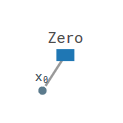
\includegraphics[]{./images/transformational_semantics_of_oz/var.png}}}%
\caption{variable as a channel}
\label{tra_var}%
\end{figure}


\section{\findex[process!operations]{Mapping operations}}
\label{sec_tra_mapping_operation}
We map \oz{} class operations to \picalc{} channels as we did with state variables. That is, we map the operations $coffee, tea, talk$  of \refFig{oz_vm_reference_name} to \picalc{} channels $coffee, tea, talk$ as shown in \refFig{tra_var2}

\section{\findex[process!data Types]{Mapping data Types}}
\label{sec_tra_mapping_data_types}
For simplicity, we do not implement any kind of type checking, but we deal with types by representing the value of the type by corresponding process. For example $cv: \{0,1,2,3\}$, means that the allowed processes to be initialized with $cv$ are: $Zero, One, Two, Three$.

\section{\findex[process!mathematical operators]{Mapping mathematical operators}}
\label{sec_tra_mapping_mathematical_operations}
\subsubsection{\findex[process!addition]{Addition}:}
\input{chapters/mainpart/transformational_semantics_oz/sections/mapping_mathematical_operations/addition}

\subsubsection{\findex[process!subtraction]{Subtraction}:}
\input{chapters/mainpart/transformational_semantics_oz/sections/mapping_mathematical_operations/subtraction}

\subsubsection{\findex[process!comparation]{Comparation}}
\input{chapters/mainpart/transformational_semantics_oz/sections/mapping_mathematical_operations/comparation}

\subsubsection{\findex[process!set union and subtraction]{Set union and subtraction}:}
The implementation of set union and abstraction processes can be found in the appendix.



\section{\findex[process!OZ class]{Mapping OZ class}}
\label{sec_tra_mapping_class}
\begin{figure}
\begin{subfigure}{.5\textwidth}
  \centering
\begin{class}{IdleShop(id: \integer)}
\begin{state}
m, vmId, self: \integer
\\t: nil | talk
\end{state} 
\\
\begin{init}
\\self = id
\\t = nil
\end{init} 
\\
\begin{op}{switch\_\_\_\_\ then\ ActiveShop}
\Delta (t)
\\x?: nil | talk
\ST
x? = t'
\end{op}
\end{class}
  \caption{1a}
  \label{fig:sfig1}
\end{subfigure}%
\begin{subfigure}{.5\textwidth}
  \centering
\fbox{  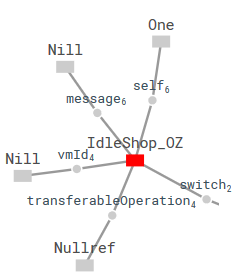
\includegraphics[width=.8\linewidth]{./images/transformational_semantics_of_oz/idleShop_OZ.png}}
  \caption{1b}
  \label{fig:sfig2}
\end{subfigure}
\vspace{2em}

\begin{subfigure}{1\textwidth}
  \centering
\lstinputlisting[backgroundcolor=\color{white},caption={ABC code: IdleShop OZ as a processes.},captionpos=b, label={idleShop_OZ}]{listings/idleShop_OZ.abc}
  \caption{1b}
  \label{fig:sfig3}
\end{subfigure}
\caption{transforming IdleShop}
\label{fig:fig}
\end{figure}

\section{\findex[process!transferable operation's variable]{Mapping transferable operation's variable}}
\label{sec_tra_mapping_transferable_operation}
As mentioned in \refSec{sec_oz_dynamic_oz}, the mobility in Dynamic \oz{} is achieved
by attaching a distinguished variable transferableOperation for location. Location transferring
is mimicked by assigning a new location to that variable. To translate the variable transferableOperation into \picalc{} we cannot use \picalc{} channel as in \refSec{sec_tra_mapping_state_variables}, since the value of transferableOperation will be a channel name and not a processes representing a value like $Zero$. Thus, we map the variable transferableOperation to a channel named transferableOperation, where:

\begin{itemize}
\item transferableOperation = nil is mapped to Nullref(transferableOperation),

\item transferableOperation = talk is mapped to Ref(transferableOperation,talk),
\end{itemize}
as shown in \refFig{tra_ref} and \refLis{tra_ref_listing}.
\input{chapters/mainpart/transformational_semantics_oz/sections/mapping_transferable_operation/ref}
Thus using the concept of transferable operation's variable we can now transform the classes \textit{IdleShop} and \textit{ActiveShop} as shown in \refFig{tra_idleShop_OZ}, \refLis{tra_idleShop_OZ_listing} and \refFig{tra_activeShop_OZ}, \refLis{tra_activeShop_OZ_listing}.
\input{chapters/mainpart/transformational_semantics_oz/sections/mapping_transferable_operation/idleShop_OZ_stargazer_ABC}
\input{chapters/mainpart/transformational_semantics_oz/sections/mapping_transferable_operation/activeShop_OZ_stargazer_ABC}

Finally, \refFig{tra_system_before}, \refFig{tra_system_after} and \refLis{tra_system_lis} show the big picture of a system consisting of two shops, a vending machine and a customer. The full implementation can be found in the appendix.
\input{chapters/mainpart/transformational_semantics_oz/sections/mapping_transferable_operation/system}



\chapter{The combination \texorpdfstring{$\pi$}{}-OZ}
\label{chp_comp_pi_oz}
This chapter study the syntactic transformation of \oz{} class into \picalc{} process. The resulting processes is intuitively defined as follow:\\


\chapter{Refinement}
\label{chp_refinement}
\begin{itemize}
\item no trace inclution implies no refenment
\item no refenment implies no simulation
\item no trace inclution implies no simulation
\end{itemize}


	% mainfile: ../Refinement.tex
\chapter{Conclusion and future work}
\label{sec_conclusion}
In this thesis we investigated the transformational semantics of the combination $\pi$-OZ for mobile processes with data.

The aim of this work is to combine the \oz{} specification with \picalc{} specification, and to transform the combination into a \picalc{} processes, in a similar way to the CSP-OZ \cite{olderog} approach. Unfortunately, we found out that the transformation is cumbersome, since the \picalc{} has only elementary constructs and is not suitable to express complex constructs like \oz{} class constructs. On the one hand, we showed how to integrate a \picalc{} process, describing the desired sequence of behavior, into an \oz{} class to form the $\pi$-OZ combination. On the other hand, we explained how to transform the combination $\pi$-OZ into a \picalc{} process through transforming \oz{} class constructs value, state variable, state schema, initial state schema and operation schema into \picalc{} processes and names accompanied by the processes of the desired sequence of behavior using the parallel operator. In spite of that, we introduced the Failure-Refinement model for \picalc{} and showed that the strong simulation does not imply the failure-refinement. Finally, we introduced the Success-Refinement model and showed that the strong simulation implies success-refinement. 

The elementary nature of the \picalc{} is a a good start for future work through introducing a state-full \picalc{}, which is an extension of the \picalc{} to support data, data types, variable and transition conditions. This will ease the mapping between \oz{} and \picalc{} constructs. Additionaly, a tool can be developed to visualize the state-full \picalc{} in a similar way to Stargazer \cite{stargazer}. Furthermore, it would be good to extend the ABC simulation-checker \cite{abc} to support simulation checking and success-refinement verification of the state-full \picalc{}. Finally, it would be interesting to extend \cite{gieseking} trace semantics to support recursive processes through developing a fixed-point algorithm for the recursive processes. This will facilitate the study of the composition properties of the Success-Refinement model, which will permit to study the possibility of introducing an Success-Divergence model and to explore its composition properties.

	\singlespacing
	%% ------------------------------------------------- Anhang -------------------------------------------------------------------
	%% Anhang
	%\appendix
	%
\section{Tabellen}
\begin{landscape}
	\begin{table}[htb]
	\caption{Credentials der PG-RiO}
	\begin{tabular}{|p{0.15\linewidth}|p{0.20\linewidth}|p{0.60\linewidth}|}
		\hline
		Zweck & Benutzername & Passwort \\
		\hline
		Dockerhub & pgrio & ~\newline \\
		\hline
		VMs & pgrio & ~\newline \\
		\hline
		SK"=Verwaltung & svadmin & ~\newline \\
		\hline
		Jenkins & pgrio & ~\newline \\
		\hline
		DB"=Writer & writer & ~\newline \\
		\hline
		DB"=Admin & admin & ~\newline \\
		\hline
		MQTT"=Datacollector & pgrio"=datacollector & ~\newline \\
		\hline
		API"=Routing & routing & ~\newline \\
		\hline
		App"=Signierung Google Playstore & \textit{Keyfile} & ~\newline \\
		\hline
	\end{tabular}
	\label{tbl:appendix:infrastruktur:cred}
	\end{table}
\end{landscape}


	%% ------------------------------------------------- Glossar ------------------------------------------------------------------
	% Glossar
	%\printglossary[style=altlist,title=Glossar]
	% Abk"urzungen
	%\deftranslation[to=German]{Acronyms}{Abk\"urzungsverzeichnis}
	%\printglossary[type=\acronymtype,style=long]
	% Symbole
	%\printglossary[type=symbolslist,style=long]
	% Englisch-Deutsch
	%\printglossary[type= translationlist, style=long]

	%% ------------------------------------------------- Literaturverzeichnis -----------------------------------------------------
	% Literaturverzeichnis
	\bibliography{bib/bib}

	%% ------------------------------------------------- Index --------------------------------------------------------------------
	% Index - Schlagworte
	\printindex
	% Index - Namensverzeichnis
	%\printindex[name]
	% Eigenst"andigkeitserkl"arung
	\newpage{}
	\pagestyle{empty}
	%\pagenumbering{} 
	\section*{Acknoldegment}
	Special thanks goes to:
	\begin{itemize}
	\item Prof. Dr. Ernst-Rüdiger Olderog for suggesting the topic of the thesis and for the continuous support.
	\item M.Sc Manuel Gieseking for providing the latex template.
	\item Dr. Emanuele D'Osualdo for support with $\pi$-calculus.
	\end{itemize}
	\selectlanguage{ngerman}
	\section*{Erkl"arung}
	Hiermit versichere ich, dass ich diese Arbeit selbstst"andig verfasst und keine anderen als die angegebenen Quellen und Hilfsmittel benutzt habe. Au"serdem versichere ich, dass ich die allgemeinen Prinzipien wissenschaftlicher Arbeit und Ver"offentlichung, wie sie in den Leitlinien guter wissenschaftlicher Praxis der Carl von Ossietzky Universit"at Oldenburg festgelegt sind, befolgt habe.
	
	\vspace{1cm}
	Oldenburg, den \today
	
	\vspace{0.5cm}
	\rule{6cm}{0.5pt}
	
	(Muhammad Ekbal Ahmad)
\end{document}
%%%  =============================================== Document END =====================================================================
